\chapter{Invasive Computing}\label{chapter:invasive computing}
\section{Job Classification}

\section{Resource Aware Programming}
In this section, we will briefly look into the details of the earlier implementations of iOpenMP and iMPI done as a part of this ongoing research project. This will give us an insight into the earlier approach taken towards realizing such resource-aware programming models and also serve as a prelude to the approach currently undertaken.

\section{Traditional Resource Management}
The role of a resource manager is to acts like a \textit{glue} for a parallel computer to execute parallel jobs. It should make a parallel computer as easy to use as almost a PC. MPI would typically be used to manage communications within the parallel program. A resource manager allocates resources within a cluster, launches and otherwise manages jobs. Some of the examples of widely used open source as well as commercial resource managers are \textbf{SLURM, TORQUE, OMEGA, IBM Platform LSF} etc. Together with a scheduler it is termed as a \textbf{\textit{Batch System}}. The Batch System serves as a middleware for managing supercomputing resources. The combination of \textit{Scheduler}$+$\textit{Resource Manager} makes it possible to run parallel jobs.\par
\noindent
\\
The role of a job scheduler is to manage queue(s) of work when there is more work than resources. It supports complex scheduling algorithms which are optimized for network topology, energy efficiency, fair share scheduling, advanced reservations, preemption, gang scheduling(time-slicing jobs) etc. It also supports resource limits(by queue, user, group, etc.). Many batch systems provide both resource management and job scheduling within a single product (e.g. LSF) while others use distinct products(e.g. Torque resource manager and Moab job scheduler). Some other examples of Job scheduling systems are \textbf{LoadLeveler, OAR, Maui, SLURM} etc.\par
\noindent
\\
\subsection{Classification}
Before the classification begins we define some terms that are used in the following.
\begin{itemize}
\item The term \textit{scheduling} stands for the process of computing a schedule. This may be done by a queuing or planning based scheduler.
\item A resource request contains two information fields: the number of requested resources and a duration for how long the resources are requested for.
\item A job consists of a resource request plus additional information about the associated application. Examples are: information about the processing environment (e. g. MPI or PVM), file I/O and redirection of stdout and stderr streams, the path and executable of the application, or startup parameters for the application. We neglect the fact that some of these extra job data may indeed be needed by the scheduler, e. g. to check the number of available licenses.
\item A reservation request is a resource request starting at a specified time for a given duration. Once the scheduler accepted such a request, it is a reservation.
\end{itemize}

We call a reservation Fix-Time request to emphasize that it can not be shifted on the time axis during scheduling. Accordingly we call a resource request Var-Time request, as the scheduler can move the request on the time axis to an earlier or later time according to the used scheduling policy. In the following we focus on resource management systems that use space-sharing.\\

The criterion for the differentiation of resource management systems is the planned time frame [42]. Queuing systems try to utilize currently free resources with waiting resource requests. Future resource planning for all waiting requests is not done. Hence, waiting resource requests have no proposed start time. Planning systems in contrast, plan for the present and future. Planned start times are assigned to all requests and a complete schedule about the future resource usage is computed and made available to the users. A comprehensive overview is given in Table 3.2 at the end of this section.\\

\textbf{\textit{Queuing Systems }}Today almost all resource management systems fall into the category of queuing systems. Several queues with different limits on the number of requested resources and the duration exist for the submission of resource requests. Jobs within a queue are ordered according to a scheduling policy, e. g. FCFS (first come, first serve). Queues might be activated only for specific times (e. g. prime time, non prime time, or weekend). The task of a queuing system is to assign free resources to waiting requests. The highest prioritized request is always the queue head. If it is possible to start more than one queue head, further criteria like queue priority or best fit (e. g. leaving less resources idle) are used to select a request. There might also exist a high priority queue whose jobs are preferred at any time. If not enough resources are available to start any of the queue heads, the system waits until enough resources become available. These idle resources may be utilized with less prioritized requests by backfilling mechanisms.\\

As the queuing systems time frame is the present, no planning of the future is done. Hence, no information about future job starts are available. Consequently guarantees can not be given and resources can not be reserved in advance. However, if participating in grid environments this functionality is desirable. Using reservations eases the way of starting a multi-site application which synchronously runs on different sites. By reserving the appropriate resources at all sites, it is guaranteed that all requested resources are available at the requested start time. With queuing systems this still has to be done manually by the administrative staff. Usually high priority queues combined with dummy jobs for delaying other jobs are used.\\

Users do not necessarily have to specify run time estimates for their jobs, as a queuing system might let jobs run to completion. Obviously users would exploit this by starting very long running jobs which then block parts of the system for a long time. Hence, run time limits were added to the queues (Table 3.1). A longer run time than the limit of the queue is not allowed and the resource management system usually kills such jobs. If the associated application still needs more CPU time, the application has to be checkpointed and later restarted by the user.\\

\textbf{\textit{Planning Systems }}Planning systems schedule for the present and future. With assigning start times to all requests a full schedule is generated. It is possible to query start and end times of requests from the system and a graphical representation of the schedule is alsopossible (Figure 3.1). Obviously duration estimates are mandatory for this planning. With this knowledge advanced reservations are easily made possible. There are no queues in planning systems. Every incoming request is planned immediately.\\

The re-planning process is the key element of a planning system. Each time a new request is submitted or a running request ends before it was estimated to end, a new schedule has to be computed and this function is invoked. At the beginning of a re-plan all non-running requests are deleted from the schedule and sorted according to the scheduling policy. Then all requests are re-inserted at the earliest possible start time in the schedule. After this step each request is assigned a planned start and end time. The non-running requests are usually stored in a list structure and different sorting criteria are applied. They define the scheduling policy of the system.\\

As planning systems work with a full schedule and assign start times to all requests, resource usage is guaranteed and advanced reservations are possible. A reservation usually comes with a given start time or if the end time is given the start time is computed with the estimated run time. When the reservation request is submitted the scheduler checks with the current schedule, whether the reservation can be made or not. That is the amount of requested resources is available from the start time and throughout the complete estimated duration. If the reservation is accepted it is stored in an extra list for accepted reservations. During the re-planning process this list is processed before the list of variable requests. It does not have to be sorted as all reservations are accepted and therefore generate no conflicts in the schedule. Furthermore, additional types of job lists are thinkable which are then integrated in the re-planning process according to their priority (reservations should have the highest and variable requests the lowest priority).\\

Controlling the usage of the machine as it is done with activating different queues for e. g. prime and non prime time in a queuing system has to be done differently in a planning system. One way is to use time dependent constraints for the planning process, e. g. “during prime time no requests with more than $75$ percent of the machines resources are placed”. Also project or user specific limits are possible so that the machine size is virtually decreased. Examples for such limitations are:
\begin{itemize}
\item Jobs requesting more than two thirds of the machine are not started during daytime, only at night and on weekends.
\item Jobs that are estimated to run for more than two days are only started at weekends.
\item It is not possible that three jobs are scheduled at the same time where each job uses one third of the machine.
\end{itemize}
If an already running request interferes with limits during its run time, it is not prematurely killed. It runs until the estimated end is reached. With the examples from above one could think of a job that requests all resources of a machine, is started on Sunday and runs until Tuesday. Such a job would then block the whole machine on Monday which contradicts the limits for Monday.\\

Planning systems also have drawbacks. The cost of scheduling is higher than in queuing systems. And as users can view the current schedule and know when their requests are planned, questions like “Why is my request not planned earlier? Look, it would fit in here.” are most likely to occur [50]. Besides the pure and easily measurable performance of the schedule (e. g. utilization or slowdown), other more social and psychologic criteria might also be considered. It might be beneficial to generate a less optimized schedule in favor of having a more understandable schedule. Furthermore, the usage of reservations should be observed, especially if made reservations are really used. Again, users tend to simply reserve resources without really needing and using them [50]. This can be avoided by automatically releasing unused reservations after a specific idle time.\\

Table 3.2 shows a summary of the previously described differences between queuing and planning based resource management systems.\\
\subsection{Job Scheduling}
\textbf{\textit{Scheduling Policies }}Typical resource management systems store requests in list-like structures. Therefore, a
scheduling policy consists of two parts: inserting a new request in the data structure at its submission and taking requests out during the scheduling. Different sorting criteria are used for inserting new requests and some examples are (either in increasing or decreasing order):
\begin{itemize}
\item by arrival time: FCFS (first come first serve) uses an increasing order. FCFS is probably the most known and used scheduling policy as it simply appends new requests at the end of the data structure. This requires very little computational effort and the scheduling results are easy to understand: jobs that arrive later are started later. With this example the term fairness is described [79]. In contrast, sorting by decreasing arrival time is not commonly used, as ’first come last served’ makes no sense in an on-line scenario with the potential risk of waiting forever (this is also called starvation). However, a stack works with decreasing order of arrival time.
\item by duration: Both increasing and decreasing orders are used. Sorting by increasing order leads to SJF (shortest job first) respectively FFIH (first fit increasing height2). Accordingly LJF (longest job first) and FFDH (first fit decreasing height) sort by decreasing run time. In an on-line scenario this requires duration estimates, as the actual duration of jobs are not known at submission time. SJF and LJF are both not fair, as very long (SJF) and short (LJF) jobs potentially wait forever. LJF is commonly known for improving the utilization of a machine.
\item by area: The jobs area is the product of the width (requested resources) and length (estimated duration). FFIA (first fit increasing area) is used in the SMART algorithm (Scheduling to Minimize Average Response Time) [91, 76]. 
\item by given job weights: Jobs may come with weights which are used for sorting. Job weights consist of user or system given weights or a combination of both. For example: all jobs receive default weights of one and only very important jobs receive higher weights, i. e. they are scheduled prior to other jobs.
\item by the Smith ratio: The Smith ratio of a job is defined by weight area and is used in the PSRS (Preemptive Smith Ratio Scheduling) algorithm [75].
\item by many others: e. g. number of requested resources, current slowdown, ...
\end{itemize}

In the scheduling process jobs are taken out of the ordered data structure for either a direct start in queuing systems or for placing the job in a full schedule (planning system):
\begin{itemize}
\item front: The first job in the data structure is always processed. Most scheduling policies use this approach as only with this a sorting policy makes sense. In queuing systems jobs might have to wait until enough resources are available. Planning systems also process the front of the data structure while placing requests as soon as possible. FCFS, SJF, and LJF use this approach.
\item first fit: The data structure is traversed from the beginning and always the first job is taken, that matches the search constraints, i. e. requests equal or less resources than currently free.
\item best fit: All jobs are tested to see whether they can be scheduled. According to a quality criterion the best suited job is chosen. Commonly the job which leaves the least resources idle in order to increase the utilization is chosen. Of course this approach is more compute intensive as the complete data structure is traversed and tested. If more than one job is best suited an additional rule is required, e. g. always take the first, the longest/shortest job, or the job with the most weight.
\item next fit: The SMART algorithm uses this approach in a special case (NFIW) [91, 76].
\end{itemize}
In general, all combinations are possible but only a few are applicable in practice. Figure 3.2 shows example schedules for FCFS, SJF, LJF, and FFIA. Sorting requests in any order while using first or best fit is not necessary, as the best job is always chosen regardless of its position in the sorted structure. However, a sorting policy could be used to choose one job, if many jobs are equal. Furthermore, best fit comes with the risk of making schedules unfair and opaque for users.\\

If fairness in common sense has to be met, i. e. the starting order equals the arrival order, only the combination of sorting by increasing arrival time and always processing the front of the job structure can be used. All other combinations do not generate fair schedules. However, such a fair scheduler is not very efficient, as jobs usually have to wait until enough free resources are available. Therefore, basic scheduling policies are extended by backfilling, a method to avoid excessive idleness of resources. Backfilling became standard in modern resource management systems today. If requests are scheduled out of their sorting order by first or best fit, some form of backfilling is carried out.

\textbf{\textit{EASY Backfilling }}The default algorithms used by current job schedulers for parallel supercomputers are all rather simple and similar to each other [37], employing a straightforward version of variable partitioning. (Recall that this means space-slicing with static-partitioning, where users specify the number of processors required by their jobs upon submittal.) In essence, schedulers select jobs for execution in first-come first-served (FCFS) order, and run each job to completion, in batch mode. The problem with this simplistic approach is that it causes significant fragmentation, as jobs with arbitrary sizes/arrivals do not pack perfectly. Specifically, if the first queued job requires many processors, it may have to wait a long time until enough are freed. During this time, processors stand idle as they accumulate, despite the fact there may very well be enough of them to accommodate the requirements of other, smaller, waiting jobs.\\

To solve the problem, most schedulers therefore employ the following algorithm. Whenever the system status changes (job arrivals or terminations), the scheduler scans the queue of waiting jobs in order of arrival (FCFS) and starts the traversed jobs if enough processors are available. Upon reaching the first queued job that cannot be started immediately, the scheduler makes a reservation on its behalf for the earliest future-time at which enough free processors would accumulate to allow it to run. This time is also called the shadow time. The scheduler then continues to scan the queue for smaller jobs (require fewer processors) that have been waiting less, but can be started immediately without interfering with the reservation. In other words, a job is started out of FCFS order only if it terminates before the shadow time and therefore does not delay the first queued job, or if it uses extra processes that would not be needed by the first queued job. The action of selecting smaller jobs for execution before their time provided they do not violate the reservation constraint is called backfilling, and is illustrated in Fig. 1.1 (see detailed description in Section 2.3).\\

This approach was initially developed for the IBM SP1 supercomputer installed at the Argonne National Laboratory as part of EASY (Extensible Argonne Scheduling sYstem), which was the first backfilling scheduler [98].1 The term “EASY” later became a synonym for FCFS with backfilling against a reservation associated with the first queued job. (Other backfill variants are described below.) While the basic concept is extremely simple, a comprehensive study involving 5 supercomputers over a period of 11 years has shown that consistent figures of 40–60 percent average
utilization have gone up to around 70 percent, once backfilling was introduced [79]. Further, in terms of performance, backfilling was shown to be a close second to more sophisticated algorithms that involve preemption (time slicing), migration, and dynamic partitioning [19, 170].\\

User Runtime Estimates The down side of backfilling is that it requires the scheduler to know in advance how long each job will run. This is needed for two reasons:
\begin{itemize}
\item to compute the shadow time for the longest-waiting job (e.g. in the example given in Fig. 1.1, we need to know the runtimes of job 1 and job 2 to determine when their processors will be freed in favor of job 3), and
\item to know if smaller jobs positioned beyond the head of the wait-queue are short enough to be backfilled (we need to make sure backfilling job 4 will not delay job 3, namely, that job 4 will terminate before the shadow time of job 3).
\end{itemize}
Therefore, EASY required users to provide a runtime estimate for all submitted jobs [98], and the practice continues to this day. Importantly, jobs that exceed their estimates are killed, so as not to violate subsequent commitments (the reservation). This strict policy has the additional benefit that it supplies an inherent and clear motivation for users to provide high quality estimates , as short enough values increase the chances for backfilling, but too-short values will get jobs prematurely killed.\\

Popularity of EASY The burden placed on users to provide estimates has not been detrimental. Rather, the combination of simplicity, effectiveness, and FCFS semantics (often perceived as most fair [123]) has made EASY a very attractive and a very popular job scheduling strategy. Nowadays, virtually all major commercial and open-source production schedulers support EASY backfilling [37], including
\begin{itemize}
\item IBM’s LoadLeveler [60, 82],
\item Cluster Resources’ commercial Moab [118] and open-source Maui [75] (which is probably the most popular scheduler used within the academia),
\item Platforms’ LSF (Load Sharing Facility) [172, 24],
\item Altair’s PBS (Portable Batch System) [68] in its two flavors: commercial PBS-Pro [33] and open-source OpenPBS [10], and
\item Sun’s GridEngine [61, 106]
\end{itemize}

The default configuration of all these schedulers, except PBS, is either EASY or plain FCFS (with FCFS, however, the schedulers’ behavior becomes EASY if backfilling is nevertheless enabled). The CTO of Cluster Resources has estimated that 90-95 percent of Maui/Moab installations do
not change their default (EASY) settings [74]. Being the exception that implies the rule, the PBS variants use Shortest-Job First (SJF) as their basic default policy. However, even with PBS, when a job is “starved” (a situation defined by PBS to occur if the job is waiting for 24 hours or more) then the scheduling reverts to EASY until this job is started. As a testament for its immense popularity, a survey about the top 50 machines within the top-500 list revealed that, out of the 25 machines for which relevant information was available, 15 (= 60 percent) were operating with backfilling enabled [36].\\

Variations on Backfilling Despite the simplicity of the concept, backfilling has nevertheless been the focus of dozens of research papers attempting to evaluate and improve the basic idea.3 We do not list them all here, but rather, cite many of them (and more) when appropriate, within
their respective contexts later on. The remainder of this section only briefly mentions some of the various tunable knobs of backfilling algorithms.\\

One tunable parameter is the number of reservations. As mentioned above, in EASY, only the first queued job receives a reservation. Thus, backfilling may cause delays in the execution of other waiting jobs which are not the first and therefore do not get a reservation [47]. The obvious
alternative is to allocate reservation to all the jobs. This approach has been named “conservative backfilling” as opposed to the “aggressive” approach taken by EASY [108]. However, it has been shown that delaying other jobs is rarely a problem, and that conservative backfilling tends
to achieve reduced performance in comparison to the aggressive alternative. The MAUI scheduler includes a parameter that allows system administrators to set up the number of reservations [75]. It has been suggested that allocating up to four reservations is a good compromise [15].\\

A second parameter is the looseness of reservations. For example, an intriguing suggestion is a “selective reservation” strategy depending on the extent different jobs have been delayed by previous backfilling decisions. If some job is delayed by too much, a reservation is made for this job [141]. This is somewhat similar to the “flexible backfilling” strategy, in which backfilling is allowed to violate the reservation(s) up to a certain slack [150, 166]. (Setting the slack in the latter strategy to be the threshold used for allocating selective reservations in the former strategy, is more or less equivalent.)\\

A third parameter is the order of queued jobs. EASY, as well as many other system designs, use FCFS order [98]. A general alternative is to prioritize jobs in a certain way, and select jobs for scheduling (including as candidates of backfilling) according to this priority order. For example, flexible backfilling combines three types of priories: an administrative priority to favor certain users or projects, a user priority used to differentiate between the jobs of the same user, and a scheduler priority used to guarantee that no job is starved [150]. The Maui scheduler has a priority function that includes even more components [75]. Another approach is to prioritize based on various job characteristics. In particular, a set of criteria related to the current queueing time and expected resource consumption of jobs has been proposed, which generalizes the well-known SJF algorithm for improved performance [174, 115] as well as combines it with fairness notions [19, 15]. The queuing order and the timing of reservations can also be determined by economic models [35] or various quality of service assurances [72].\\

A fourth parameter (related to the previous one) is the partitioning of reservations. The processors of a machine can be partitioned into several disjoint sets (free processors can dynamically move around between them based on current needs). Each set is associated with its own wait-queue and reservation. Lawson and Smirni divided the machine such that different sets serve different jobs classes, characterized by their estimated runtime (e.g. short, medium, and long) [90, 92]. A backfilling candidate is chosen in a round-robin fashion, each time from a different set, and must respect all reservations. By separating short from long jobs, this multiple queue policy reduces the likelihood that a short job is overly delayed in the queue behind a very long job, and therefore improves average performance metrics.\\

A fifth parameter is the adaptiveness of backfilling. An adaptive backfill scheduler continuously simulates the execution of recently submitted jobs under various scheduling disciplines, compares the hypothetical resulting performance, and periodically switches the scheduling algorithm
to be the one that scored the highest. In the face of different workload conditions, this adaptiveness has the effect of both improving and stabilizing the observed performance results [144, 149].\\

A sixth parameter is the amount of lookahead into the queue. Most backfilling algorithms consider the queued jobs one at a time when trying to backfill them, which often leads to loss of resources to fragmentation. The alternative is to consider the whole queue at once, and try to
find the set of jobs that together maximize the utilization while at the same time respecting the allocated reservation(s). This appears to be a NP-hard problem, but due to the fact machine sizes are relatively small, this can be done in polynomial time (in the complexity of the machine size) using dynamic programming, leading to optimal packing [132, 131].\\

A seventh and final parameter is related to speculative backfilling, where the scheduler is allowed to exploit gaps in the schedule for backfilling, even if the backfilled job interferes with the reservation. By doing so, the scheduler speculates that the backfilled job would terminate sooner than its estimate suggests, and in any case before the shadow time. Successful speculations obviously improve performance and utilization, and have no negative side effects. But unsuccessful speculations must somehow be dealt with. Unfortunately, all previously suggested solution resulted in a scheduling algorithm that lies outside the attractive variable partitioning domain: The simplest alternative is to kill the offending backfilled job and restart it later on [90]. A similar idea is to employ “short test runs”, during which jobs either manage to terminate, or are reinserted to the wait-queue with a tighter estimate deduced from the test [115, 15]. Unfortunately, both ideas assume jobs are restartable, which is often not the case. A possible workaround is to employ preemption (time sharing), such that instead of killing and restarting the job, it is suspended and kept in memory, only to be resumed later on from the point in which it was stopped [139]. However, if preemption comes into play, it may be preferable to instead combine backfilling with a full fledged gang scheduler altogether [169]. This combination has even been further extended by adding migration capabilities [85, 170]. A recent study suggested preemption is actually redundant if migration or dynamic partitioning are available. The idea is to reduce the backfilled job’s processor allocation by folding it over itself. This frees most of its processors, and limits the performance degradation to the offending job [162].\\

Finally, a new direction in job scheduling research is to try and minimize the electric power demand, which is rapidly becoming a problem in the context of supercomputing [129]. It has been suggested to integrate the concept of scheduling and power management within EASY [91]. The proposed scheduler continuously monitors load in the system and selectively puts certain nodes in “sleep mode” (makes them unavailable for execution), after estimating the effect of fewer nodes on the projected job slowdown. Using online simulation, the system adaptively selects the minimal number of processors that are required to meet certain negotiated service level agreements.
\subsection{SLURM}
The prime focus of this work will be on \textbf{SLURM(Simple Linux Utility For Resource Management)} which will be the choice of batch system upon which the support for Invasive Computing will be demonstrated. SLURM is a sophisticated open source batch system with about 500,000 lines of C code whose development started in the year 2002 at Lawrence Livermore National Laboratory as a simple resource manager for Linux Clusters and a few years ago spawned into an independent firm under the name SchedMD. SLURM has since its inception also evolved into a very capable job scheduler through the use of optional plugins. It is used on many of the world's largest supercomputers and is used by a large fraction of the world's TOP500 Supercomputer list. It supports many UNIX falvors like AIX, Linux, Solaris and is also fault tolerant, highly scalable, and portable.\par
\noindent
\\
\textbf{Plugins} are dynamically linked objects loaded at run time based upon configuration file and/or user options. \ref{fig:6} shows where these plugins fit inside SLURM. Approximately $80$ plugins of different varities are currently available. Some of them are listed below:\\
\begin{itemize}
\item \textbf{\textit{Accounting storage:}} MySQL, PostgreSQL, textfile.
\item \textbf{\textit{Network Topology:}} 3D-Torus, tree.
\item \textbf{\textit{MPI:}} OpenMPI, MPICH1, MVAPICH, MPICH2, etc.
\end{itemize}
PLugins are typically loaded when the daemon or command starts and persist indefinitely. They provide a level of indirection to a configurable underlying function.
\begin{figure}[h]
\centering
%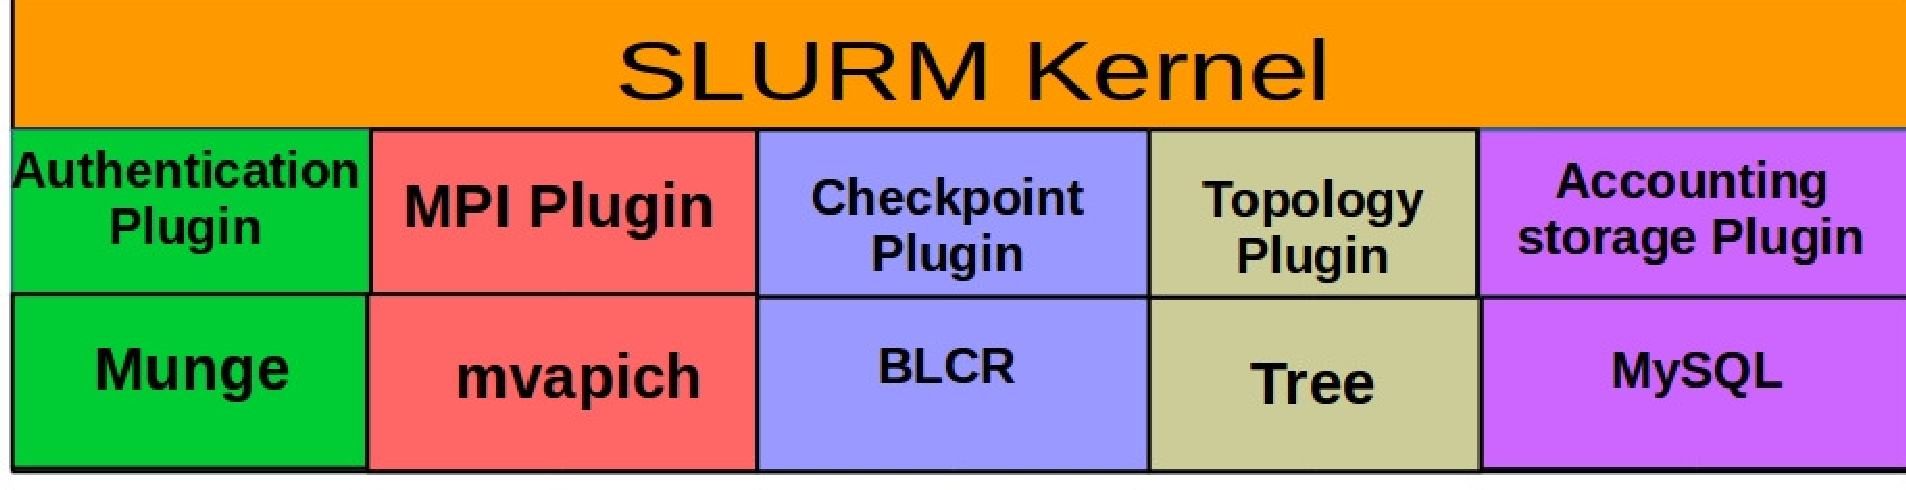
\includegraphics[width=1.0\textwidth]{./figures/plugin.pdf}
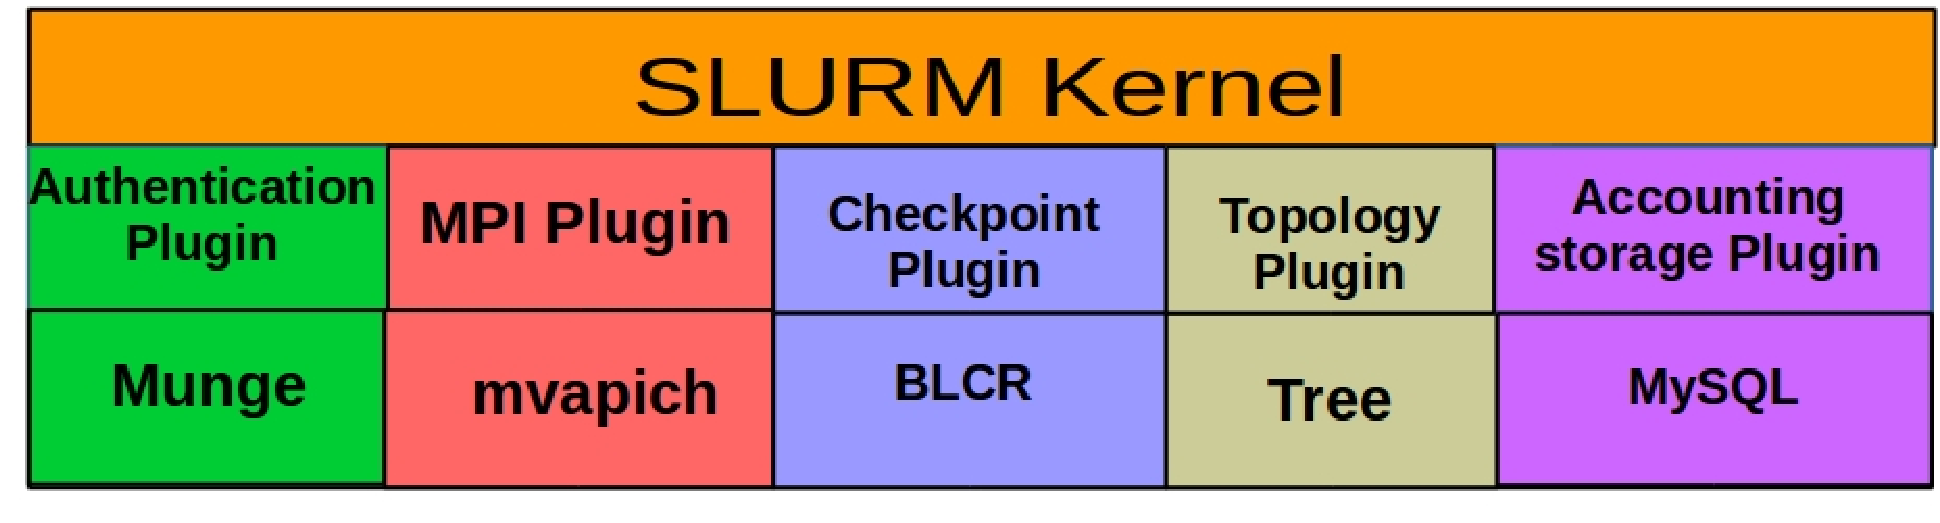
\includegraphics[width=1.0\textwidth]{./figures/plugin.eps}
\vspace{-0.15in}
\caption{SLURM with optional Plugins}
\label{fig:6}
\end{figure}


\section{Invasive Resource Management}
\subsection{Invasive MPI}
Message Passing has for long remained the dominant programming model for distributed memory systems. MPI stands for Message Passing Interface. It is a standardized and portable message passing system designed to function on a wide variety of parallel computers. It defines the syntax and semantics of a core of library routines for writing portable programs in C, C++ and Fortran. It implements a message passing type of parallel programming model where the application consists of a set of processes with separate address spaces. The processes exchange messages by explicit send/receive operations. There are several well-tested and efficient implementations of MPI, many of which are open-source or in the public domain. These have fostered the development of a parallel software industry, and encouraged development of portable and scalable large-scale parallel applications.\\ 

In the context of invasive computing, parallel applications are resource aware and will invade or retreat from resources depending on their availability and on the load imbalances encountered during their runtime. To support this, some form of dynamic process management of the parallel application is necessary. And, in order to realize this in practice, the most basic requirement would be the need of a library that will serve as an application programming interface for programmers to implement such invasic applications that are capable of adapting to a changing set of resources. \\

The original MPI computational model was static in terms of the number of processes. Dynamic processes support was later added in version 2.0 of the standard in the form of MPI{\_}COMM{\_}SPAWN and its related operations. The spawn operation creates new processes in a separate child process group, whereas the callers belong to the parent process group. The callers, or parents, block in the spawn operation, while the resource manager creates the new children processes. The two process groups are connected to each other via an intercommunicator which is generated during this spawn process and returned to the application. This intercommunicator can then be used to reach children processes from the parent's process group, or parent processes from the children's process group. Another form of spawn is the multiple version which allows the callers to specify multiple binaries to start as children processes. Additional operations were also introduced so that applications could start independently and later connect their process groups, such as: MPI{\_}OPEN{\_}PORT, MPI{\_}PUBLISH{\_}NAME, MPI{\_}OPEN{\_}PORT, MPI{\_}LOOKUP{\_}NAME, MPI{\_}COMM{\_}ACCEPT and MPI{\_}COMM{\_}CONNECT. \\

Although the MPI standard provides support for dynamic processes, it suffers from many drawbacks as mentioned below:
\begin{itemize}
\item The spawn operations are collective operations and are synchronous across both the parent and child process groups. This effects performance and can induce delays of several seconds.
\item These operations produce intercommunicators based on disjoint process groups. Subsequent creation of processes result in multiple disjoint process groups. These factors can complicate the development of an MPI application.
\item Destruction of processes can be done only on entire process groups. This shortcoming limits the granularity of operations that can be carried out as only entire process groups can be destroyed. This also limits the location of the resources that the application can release at runtime.
\item The processes created with spawn are typically run in the same unmodified resource allocation. Although, not a limitation of the standard itself, but, lack of support from resource manager will result in limiting the usefulness of this spawn operation by not changing the physical resource set of the application.
\end{itemize}


\subsection{Resource Management Extensions}
Existing batch systems usually only support static allocation of resources to applications before job start. Hence we need some kind of an Invasive Resource Management to be integrated into these existing batch systems so that we can support malleable jobs allowing us to change the allocated resources dynamically at runtime. In order to achieve this we will follow the below approach:
\begin{itemize}
\item \textbf{\textit{Invasive Resource Manager (alias iRTSched):}} An independent component which will talk to the current batch systems via a communication mechanism(protocol) to obtain invasive job(s) submitted specifically to the invasic partition that can support invasive computing. The iRTSched will then take these jobs and perform some kind of runtime scheduling for pinning these jobs to the resources in the partition and makes these decisions in order to optimize certain local metrics such as resource utilization, power stability, energy efficiency etc. The scheduling here is done at the granularity of cores and sockets. iRTSched is the one that has the complete information of the resources in the invasic partition and also manages them. This component in an independent entity with the purpose of inter-operating with existing batch systems rather than replacing them with an entirely new one. It may be possible that in the future this component will not be a separate entitiy but will be built into the batch system itself.
\item \textbf{\textit{Invasive Batch Job Scheduler (alias iBSched):}} This component will be a new extension built into the existing batch systems for performing job scheduling. The scheduling decisions are communicated via the protocol used to speak to iRTSched and these decisions are basically job(s) selected via a scheduling algorithm to be submitted to the iRTSched for execution. The scheduling decisions will be made on the basis of available resources in the partition and it is the iRTSched that communicates this to iScheduler in the form of resource offers (Real/Virtual). It can be a virtual resource offer because the iRTSched can hide the real resources and present a rather fake view of them to iScheduler in the hope of getting a mapping of jobs to offer that is more suitable to satisfy its local metrics. Similar to iRTSched, the iScheduler makes its decisions to optimize for certain local metrics such as high job throughput, reduced job waiting times, deadlines, priorities etc. This highlights the mismatching policies/metrics for which both the iRTSched and iScheduler make their decisions on and hence both will be involved in some kind of a negotiation via the protocol to reach a common agreement.
\item \textbf{\textit{Negotiation Protocol:}} This protocol forms the core of the interaction between the iScheduler and iRTSched. It allows for iRTSched to make one or a set of resource offers to iScheduler which then needs to select jobs from its job queue to be mapped to these resource offers and finally sent back to the iRTSched. The iRTSched will then decide whether to accept/reject this mapping to satisfy its local metrics. If it accepts it will launch them based on some run time scheduling and if it rejects then it informs this to iScheduler in addition to sending it a new resource offer. The iScheduler can also reject the resource offers in which case it will be sent a new one. On accepting an offer, the iScheduler then repeats its tasks to send back a mapping to iRTSched and this interaction continues until both reach a common agreement. If the number of such attempts reach a threshold then iScheduler will just accept whatever offer it receives and iRTSched will also accept whatever Map:Jobs$\rightarrow$Offers it receives closing this transaction of negotiating. After this a new transaction will start.
\item \textbf{\textit{SLURM:}} SLURM is our choice of an existing batch system upon which this new implementation will be demonstrated as a proof of concept to support the new paradigm of resource-aware programming in the domain of invasive computing. In the near future, This can motivate further such supporting infrastructures with other batch systems using such Invasive Resource Management and Scheduling components.
\end{itemize}
\noindent
This project implements a testing prototype for demonstrating how such an approach to support invasive computing with the above entities may work. It will involve implementing the communication infrastructure using SLURM API due to which iRTSched and iScheduler will interact with each other using protocol messages filled with dummy values. It will also involve implementing the iScheduler as a new plugin(multithreaded) for SLURM and iRTSched as a fake multithreaded Invasive Resource Manager daemon with bare minimum functionalities that in the near future will be an enhanced version of the daemon slurmd(built on top of it) found in SLURM. For the purposes of testing this prototype, the different scenarios that can be observed most of the time with the kind of negotiation protocol described earlier would be verified.
